\documentclass[aspectratio=169]{beamer}
\usepackage[russian]{babel}
\usepackage[utf8]{inputenc}
\usepackage{verbatim}
\usepackage{graphicx}
\usepackage{pgfpages}
\usepackage{ulem}
\usepackage{float}
\usepackage{amsmath}

\setbeamercolor{title}{fg=white}
\setbeamercolor{author}{fg=white}
\setbeamercolor{normal text}{fg=black}
\setbeamercolor{frametitle}{fg=black}
\setbeamercolor{item}{fg=red}
\setbeamercolor{block title}{fg=red}
\setbeamercolor{section in toc}{fg=red}
\setbeamercolor{footline}{fg=white}
\setbeamercolor{title in head/foot}{fg=white,bg=black}

\setbeamertemplate{navigation symbols}{}
\setbeamertemplate{headline}{
    
\includegraphics[height=1mm, width=\paperwidth]{wg-headline.png}
}

\setbeamertemplate{footline}{
    \begin{beamercolorbox}[ht=1.2em]{title in head/foot}
        {\footnotesize \hspace{1em}\inserttitle, \insertshortauthor}
    \end{beamercolorbox}
}


\begin{document}

\title{Очереди сообщений в распределённых системах}
\author{Максим Мельников (max\_posedon)}
\date{}

{

\title{
    
\includegraphics[width=0.5\textwidth]{wg-logo.png}\\
    {\Huge ОЧЕРЕДИ СООБЩЕНИЙ\\В РАСПРЕДЕЛЁННЫХ СИСТЕМАХ}
}
\author{МАКСИМ МЕЛЬНИКОВ (MAX\_POSEDON)}

\usebackgroundtemplate{
\includegraphics[width=\paperwidth]{wg-end.jpg}}
\begin{frame}[plain]{}
    \titlepage
\end{frame}

}

\usebackgroundtemplate{
\includegraphics[width=\paperwidth]{wg-bg.jpg}}
\logo{
    
\includegraphics[height=1.7cm]{wg-logo.png}
}

\begin{frame}{КТО Я}
    \begin{itemize}
        \item Wargaming.net
            \begin{itemize}
                \item \sout{Order of War}
                \item \sout{Order of War: Challenge}
                \item World of Tanks developer
            \end{itemize}
        \item Linux Mobile hobbyist
            \begin{itemize}
                \item \sout{Openmoko}
                \item systemd
                \item telepathy
                \item Gentoo
            \end{itemize}
    \end{itemize}
    \note{
    Сначала немного о себе. В компанию я пришёл 3.5 года назад, на проект Order of War.
Там я занимался выделением standalone "игрового сервера" и портированием его на Linux.

    После релиза Order of War: Challenge, перешёл на проект World of Tanks, 
где поработал над: поддержкой AMQP для игрового сервера; разработкой клановых войн; 
а также разработкой Wargaming.net ID (OpenID) сервиса.

    Кроме работы, меня интересует тема OpenSource и Linux-а на мобильных устройствах,
особенно всё, что касается systemd, telepathy и такого дистрибутива как Gentoo.
    }
\end{frame}

\frame{
    \frametitle{ОЧЕРЕДИ СООБЩЕНИЙ}
    \begin{block}{Что это такое?}
    Это архитектура и ПО промежуточного уровня, которое занимается сбором, хранением 
    и маршрутизацией (распределением) сообщений между компонентами. 
    \end{block}

    \begin{block}{Зачем?}
    Организация очереди сообщений помогает раз-балансировать нагрузку между различными узлами сети, 
    избавиться от единой точки отказа (SPOF),
    выполнять бизнес-логику приложения асинхронно, 
    повысить скорость ответа системы и многое другое.
    \end{block}
}

\frame{
    \frametitle{Apache ActiveMQ}
    \begin{itemize}
    \item Реализован на Java
    \item Полностью реализует Java Message Service 1.1 (JMS)
    \item "Enterprise Features": кластеризация, журнал операций, ...
    \end{itemize}
}

\frame{
    \frametitle{ZeroMQ}
    \begin{itemize}
    \item Реализован на C++
    \item Работает без сервера
    \item Низкоуровневое API
    \end{itemize}
}

\frame{
    \frametitle{PgQ}
    \begin{itemize}
    \item Реализован на C/SQL как расширение к PostgreSQL
    \item Тесная интеграция с базой данных (транзакции)
    \item Skype
    \end{itemize}
}

\frame{
    \frametitle{AMQP}
    \begin{block}{AMQP}
    Advanced Message Queueing Protocol   
    \end{block}

    \begin{block}{Apache Qpid}
    \begin{itemize}
    \item Реализация на C++
    \item RedHat
    \end{itemize}
    \end{block}

    \begin{block}{RabbitMQ server}
    \begin{itemize}
    \item Реализация на Erlang
    \item VMWare
    \end{itemize}
    \end{block}
}

\frame{
    \frametitle{ТЕРМИНОЛОГИЯ}
    \begin{itemize}
    \item Сообщение (mesasage)
    \item Точка обмена (exchange)
    \item Очередь (queue)
    \item Ключ маршрутизации (routing key)
    \end{itemize}
}

\frame{
    \frametitle{Hello World}
    \begin{figure}[htb]
    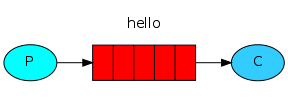
\includegraphics[width=\textheight]{hello.png}
    \end{figure}
}

\frame{
    \frametitle{Work queues}
    \begin{figure}[htb]
    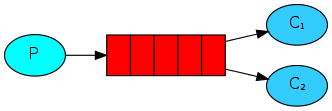
\includegraphics[width=\textwidth]{queues.png}
    \end{figure}
}

\frame{
    \frametitle{Publish/Subscribe}
    \begin{figure}[htb]
    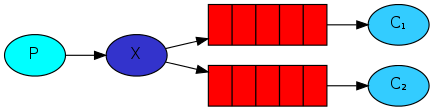
\includegraphics[width=\textwidth]{pubsub.png}
    \end{figure}
}

\frame{
    \frametitle{Routing}
    \begin{figure}[htb]
    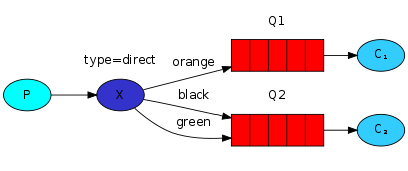
\includegraphics[width=\textwidth]{routing.png}
    \end{figure}
}

\frame{
    \frametitle{Topics}
    \begin{figure}[htb]
    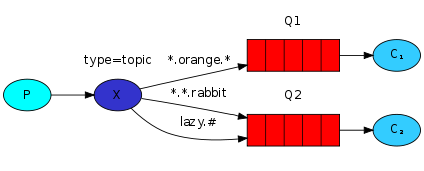
\includegraphics[width=\textwidth]{topics.png}
    \end{figure}
}

\frame{
    \frametitle{RPC}
    \begin{figure}[htb]
    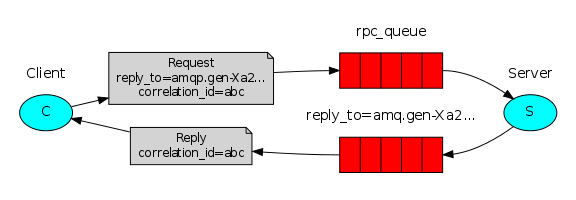
\includegraphics[width=\textwidth]{rpc.png}
    \end{figure}
}

{
\setbeamertemplate{footline}{}

\setbeamercolor{frametitle}{fg=white}
\setbeamercolor{normal text}{fg=white}
\setbeamercolor{block title}{fg=white}
\setbeamercolor{block body}{fg=red}

\usebackgroundtemplate{
\includegraphics[height=\paperheight]{wg-end.jpg}}
\begin{frame}{СПАСИБО ЗА ВНИМАНИЕ. ВОПРОСЫ}
    \begin{block}{Максим Мельников}
    \par \url{http://www.rabbitmq.com/getstarted.html}
    \par \url{mailto:m\_melnikau@wargaming.net}
    \par \url{https://plus.google.com/114669104565190507739/}
    \par \url{https://twitter.com/max\_posedon}
    \par \url{http://wargaming.com}
    \end{block}
\end{frame}
}

\end{document}

